\chapter{Deep Reinforcement Learning (DRL)}\label{Deep Reinforcement Learning (DRL)}

\section*{Intro \cite{drl-1}}

\begin{table}[H]
    \begin{minipage}{0.45\linewidth}
        \begin{figure}[H]
            \centering
            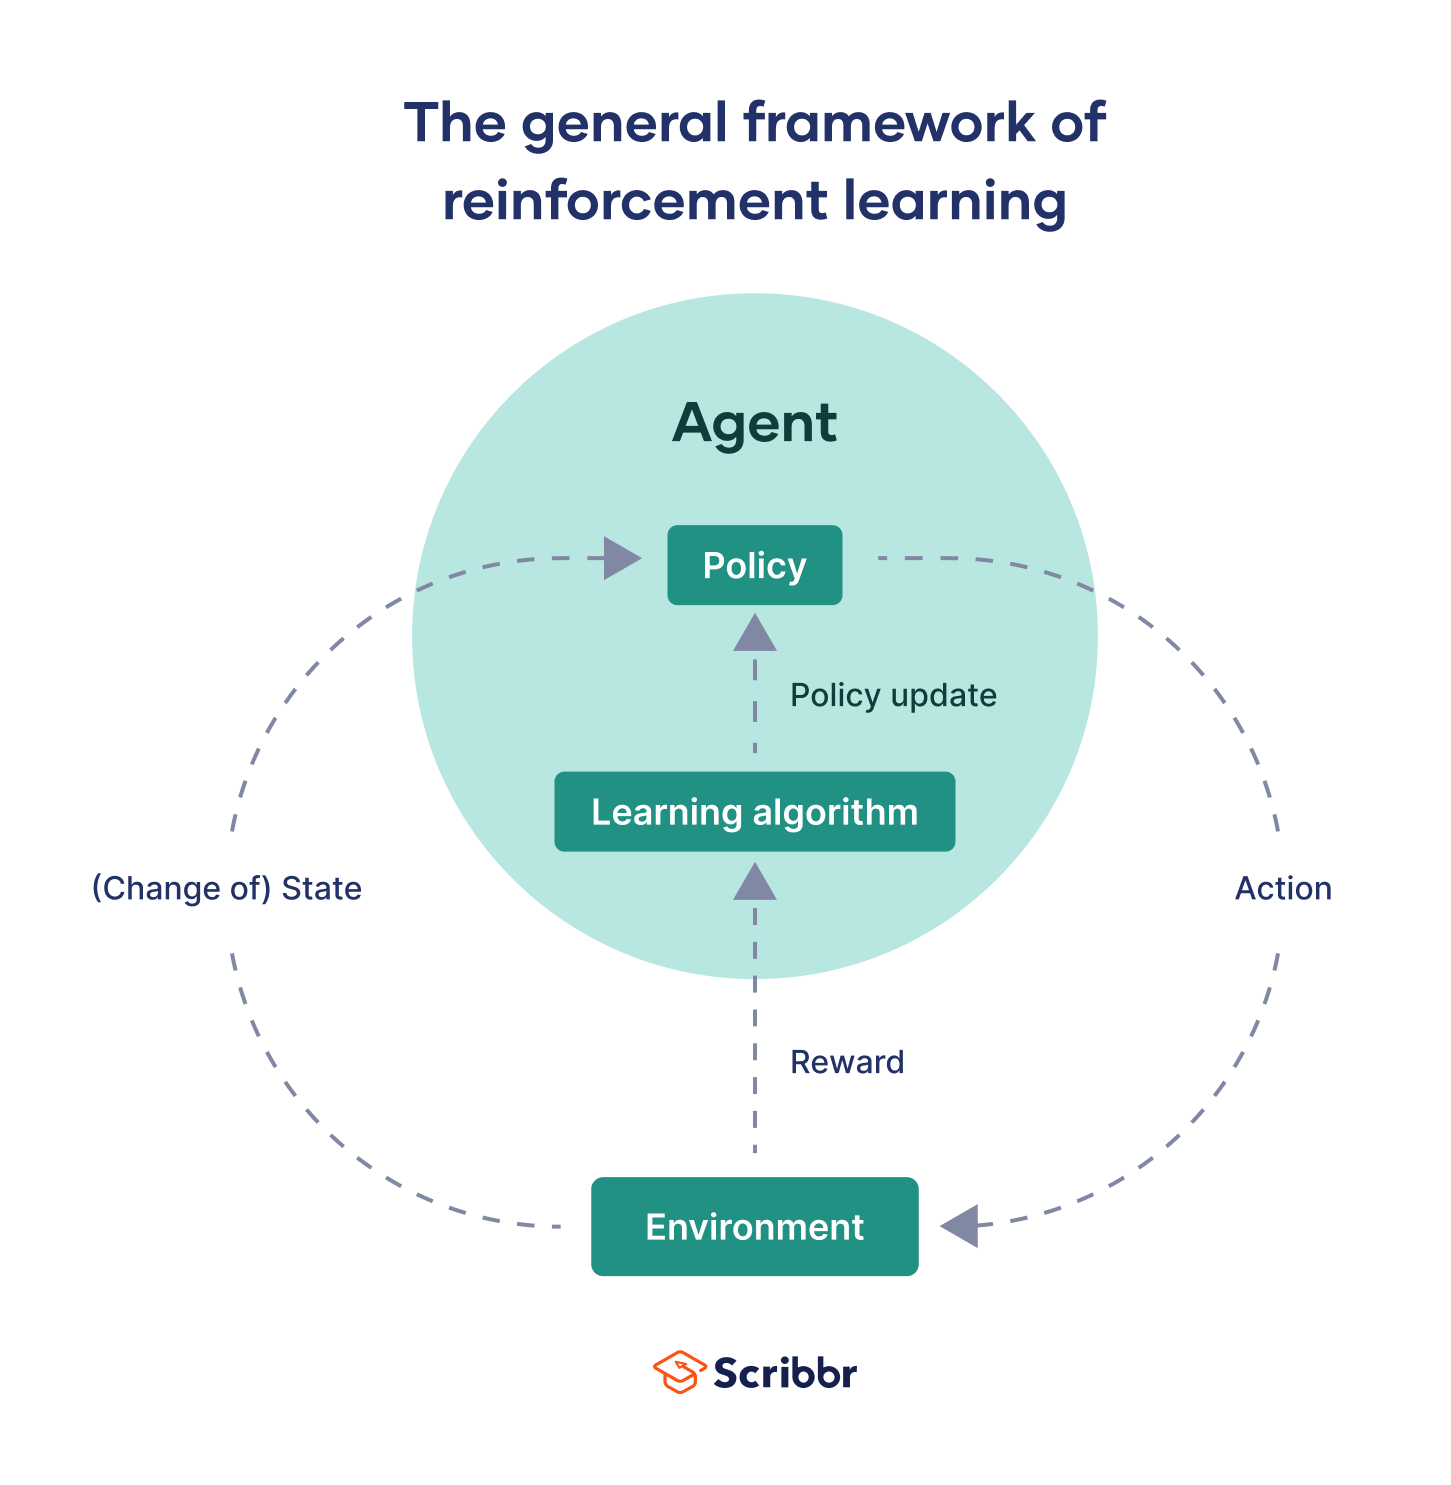
\includegraphics[height=7cm]{Pictures/deep-reinforcement-learning/drl-flow.jpg}
            \caption{Deep Reinforcement Learning}
        \end{figure}        
    \end{minipage}
    \hfill
    \begin{minipage}{0.45\linewidth}
        “\textbf{Reinforcement learning}” to refer to decision-making with uncertain models, and in addition, current actions alter the future behavior of the system. Therefore, if the same action is taken at a future time, the consequences might not be the same. This additional feature distinguishes RL from “mere” decision-making under uncertainty.\cite{arxiv-2304.00803}
    \end{minipage}
\end{table}





\section{Components of a RL \cite{medium-numsmt2-rl-ch1-part-1}}\label{Components of a RL}
\begin{enumerate}[itemsep=5pt]
    \item \textbf{Agent/ Actor}: The agent is the thing that is acting.\\ For example, in a video game it could be the character that is being controlled, in robotics it could be a robotic arm, etc.
    
    \item \textbf{Environment}: The environment is where the agent is acting. \\ This could be a video game like chess in which the agent is able to observe the positions of its own pieces as well as the positions of the opponent’s pieces. \\ For things like self-driving cars, their environment could be the real-world in which the agent (the car) is able to observe traffic signals, pedestrians and other cars.
    
    \item \textbf{States}: The state is simply another word for the observation returned from the environment. \\ In the chess example, a formal representation of the state of the game might be a list of all the pieces and their positions on the board.
    
    \item \textbf{Reward}: Reward defines the goal of the problem. The reward is given to the agent from the environment to encourage or punish certain behaviors. \\ A chess agent could get small positive rewards for doing things like taking opponent’s pieces and a big positive reward for winning the game. \\ A self-driving car could get negative rewards for doing things like crashing or disobeying traffic laws.

    \item \textbf{Value Function}: While the reward defines what’s good in the short-term, value functions define what’s good in the \textbf{long-term}. They do this by calculating the value of being in a particular state from the perspective of maximizing cumulative reward (the total reward the agent will receive over time). In complex environments, it may be better to forgo short-term rewards in exchange for greater long-term reward (similar to delayed-gratification).

    \item \textbf{Actions}: The agent must have the ability to influence the environment and it does so by taking actions.\\ An action could be moving a game piece to a new position on the board or increasing the velocity of a car.

    \item \textbf{Policy} ( $\pi$ )\indexlabel{DRL: Policy}: The policy defines the way the agent behaves. Given an observation from the environment, the policy determines which actions the agent should take. As the agent gains experience it tries to improve it’s policy to get greater cumulative rewards.
\end{enumerate}



































